
\documentclass[12pt,a4paper]{article}

% ------------------------------------------------------------
% Fonts & layout
% ------------------------------------------------------------
\usepackage[T1]{fontenc}
\usepackage[utf8]{inputenc}
\usepackage{lmodern}
\usepackage{microtype}
\usepackage{geometry}
\geometry{margin=1in}
\usepackage{array}
\usepackage{booktabs}

% ------------------------------------------------------------
% Math
% ------------------------------------------------------------
\usepackage{amsmath,amssymb,amsthm,mathtools}

% Standard operators
\DeclareMathOperator{\id}{id}
\DeclareMathOperator{\im}{im}
\DeclareMathOperator{\coker}{coker}
\DeclareMathOperator{\Hom}{Hom}

\DeclareMathOperator{\Spec}{Spec}
\DeclareMathOperator{\Proj}{Proj}

% Categories / notation
\newcommand{\Ab}{\mathbf{Ab}}
\newcommand{\PreSh}{\mathbf{PreSh}}
\newcommand{\Sh}{\mathbf{Sh}}

\newcommand{\F}{\mathcal F}


% basic number sets
\newcommand{\RR}{\mathbb{R}}

% sheaf letters

\newcommand{\G}{\mathcal G}

\newcommand{\GG}{\mathbb G}


\newcommand{\AffSch}{\mathbf{AffSch}}
\newcommand{\ZZ}{\mathbb Z}

\newcommand{\PP}{\mathbb P}

\usepackage{tikz}
\usetikzlibrary{decorations.pathreplacing}
\usetikzlibrary{positioning,arrows.meta}

% sheaf of continuous real-valued functions
\newcommand{\Czero}{\mathcal C^0}        % “C^0”
\newcommand{\CzeroX}{\mathcal C^0_X}     % sheaf on X (optional)

\newcommand{\Cinfty}{\mathcal C^\infty}
\newcommand{\CinftyM}{\mathcal C^\infty_M} % if you use C^\infty_M

% number sets / standard symbols
\newcommand{\CC}{\mathbb{C}}

% structure sheaf notation in complex geometry
\newcommand{\OO}{\mathcal{O}}
\newcommand{\OOX}{\mathcal{O}_X} % optional convenience



\newcommand{\Sch}{\mathrm{Sch}}
\newcommand{\Rings}{\mathrm{Rings}}

\newcommand{\kappares}{\kappa}
\newcommand{\GammaX}{\Gamma(X,\mathcal O_X)}

\newtheorem{theorem}{Theorem}[section]
\newtheorem{proposition}[theorem]{Proposition}
\newtheorem{lemma}[theorem]{Lemma}

\newcommand{\nilrad}{\sqrt{(0)}}

\newcommand{\Frac}{\operatorname{Frac}}
\newcommand{\codim}{\operatorname{codim}}
\newcommand{\trdeg}{\operatorname{trdeg}}

\newcommand{\height}{\operatorname{height}}

\newcommand{\Pic}{\operatorname{Pic}}
\newcommand{\divisor}{\operatorname{div}}

\newcommand{\Z}{\mathbb{Z}}
\newcommand{\Cl}{\operatorname{Cl}}

\providecommand{\Spec}{\operatorname{Spec}}
\providecommand{\A}{\mathbb A}
\providecommand{\Pj}{\mathbb P}
\providecommand{\G}{\mathbb G}

% ------------------------------------------------------------
% Links
% ------------------------------------------------------------
\usepackage{xcolor}
\usepackage{hyperref}
\usepackage{bookmark}
\hypersetup{
  colorlinks=true,
  linkcolor=blue!50!black,
  urlcolor=blue!50!black,
  citecolor=blue!50!black,
  pdftitle={Algebraic Geometry 14
  },
  pdfauthor={},
  pdfsubject={Lecture notes (reorganized)},
  pdfcreator={TeXStudio / LaTeX}
}

% ------------------------------------------------------------
% Diagrams
% ------------------------------------------------------------
\usepackage{tikz-cd}

% ------------------------------------------------------------
% Lists
% ------------------------------------------------------------
\usepackage{enumitem}
\setlist[itemize]{topsep=4pt,itemsep=2pt,parsep=0pt,partopsep=0pt}
\setlist[enumerate]{topsep=4pt,itemsep=2pt,parsep=0pt,partopsep=0pt}

% ------------------------------------------------------------
% Theorem environments
% ------------------------------------------------------------
\newtheoremstyle{notespace}{6pt}{6pt}{\normalfont}{}{\bfseries}{.}{0.5em}{}
\theoremstyle{notespace}
\newtheorem{definition}{Definition}[subsection]

\newtheorem{corollary}[definition]{Corollary}
\newtheorem{remark}[definition]{Remark}
\newtheorem{example}[definition]{Example}
\newtheorem{warning}[definition]{Warning}


\DeclareMathOperator{\Log}{Log}

\newcommand{\B}{\mathcal B}
\newcommand{\C}{\mathcal C}
\newcommand{\Ocal}{\mathcal O}
\newcommand{\I}{\mathcal I}


\newcommand{\Fp}{\mathcal F'}      % subsheaf
\newcommand{\Fpp}{\mathcal F''} 

\newcommand{\GammaU}[1]{\Gamma(U,#1)}

\DeclareMathOperator*{\colim}{colim}

% circle
\newcommand{\SSone}{S^1}


\usetikzlibrary{arrows.meta,positioning,calc,shapes.geometric,fit}

\usepackage{adjustbox}

% sheaves of continuous functions


% ------------------------------------------------------------
% Paragraph spacing
% ------------------------------------------------------------
\setlength{\parskip}{0.5em}
\setlength{\parindent}{0pt}

\setcounter{tocdepth}{2}
\setcounter{secnumdepth}{2}

% ------------------------------------------------------------
% Fancy headers
% ------------------------------------------------------------
\usepackage{fancyhdr}
\pagestyle{fancy}
\fancyhf{}
\lhead{Theory of Algebraic Geometry 14}
\rhead{\thepage}
\renewcommand{\headrulewidth}{0.4pt}
\setlength{\headheight}{14.5pt}




\begin{document}


\title{Algebraic Geometry 14\\
	\large Riemann surfaces}
\author{}
\date{}

	\maketitle
	

	\setcounter{section}{0}

\tableofcontents

	\clearpage
	
\section{Problem 8: Monodromy Group of a Branched Covering}

\textbf{Problem.}

Let \(f:R\to S\) be an analytic map of compact Riemann surfaces, and
\(B\subset S\) the set of branch points. Given a point
\(P\in S\setminus B\), explain how a closed curve \(\gamma\) in
\(S\setminus B\) starting and ending at \(P\) defines a permutation of
the finite set \(f^{-1}(P)\). Show that the group obtained from all such
closed curves is a transitive subgroup of the full symmetric group of
the fibre \(f^{-1}(P)\).

\emph{Recall that}
\[
R\setminus f^{-1}(B)\to S\setminus B
\]
\emph{is a regular covering map.}

Determine this subgroup when
\[
f:\mathbb C_\infty\to\mathbb C_\infty,
\qquad
f(z)=z^3-3z+1.
\]

\bigskip

\textbf{Solution.}

Choose a point
\[
P\in S\setminus B.
\]

Since
\[
f:R\setminus f^{-1}(B)\longrightarrow S\setminus B
\]
is a covering map, every loop
\[
\gamma:[0,1]\to S\setminus B,
\qquad
\gamma(0)=\gamma(1)=P,
\]
lifts uniquely once a starting point in the fibre
\[
f^{-1}(P)=\{Q_1,\ldots,Q_n\}
\]
has been chosen.

For each \(Q_i\), let \(\widetilde{\gamma}_i\) be the lift of
\(\gamma\) beginning at \(Q_i\). Since \(\gamma\) is closed, the endpoint
of \(\widetilde{\gamma}_i\) again lies in \(f^{-1}(P)\). Therefore
\(\gamma\) determines a permutation
\[
\sigma_\gamma:f^{-1}(P)\to f^{-1}(P).
\]

The set of all such permutations forms a subgroup
\[
G\subseteq S_{f^{-1}(P)},
\]
called the \emph{monodromy group} of the covering.

Since \(R\setminus f^{-1}(B)\) is connected, the covering is connected.
Hence the monodromy action is transitive. Therefore \(G\) is a
transitive subgroup of the symmetric group of the fibre.

Now consider
\[
f:\mathbb C_\infty\to\mathbb C_\infty,
\qquad
f(z)=z^3-3z+1.
\]

We compute
\[
f'(z)=3z^2-3=3(z-1)(z+1).
\]

Hence the critical points are
\[
z=1,
\qquad
z=-1.
\]

The corresponding branch values are
\[
f(1)=1-3+1=-1,
\]
and
\[
f(-1)=-1+3+1=3.
\]

Since \(f\) is a polynomial of degree \(3\), there is also a branch value
at infinity. Thus
\[
B=\{-1,3,\infty\}.
\]

A generic fibre has three points. Around each finite branch point,
exactly two sheets come together, so the local monodromy is a
transposition. Therefore the monodromy group is generated by two
transpositions.

Because the covering is connected, the monodromy group acts transitively
on the three points of a generic fibre. The only transitive subgroup of
\(S_3\) generated by transpositions is \(S_3\) itself.

Hence
\[
G=S_3.
\]

Therefore the monodromy group of
\[
f(z)=z^3-3z+1
\]
is
\[
\boxed{S_3}.
\]

\bigskip

\hrule

\bigskip

\section{Problem 9: Conformal Equivalence of Complex Tori}

\textbf{Problem.}

Let \(f\) and \(F\) be as in Question 7 and suppose that \(f\) is a
conformal equivalence. Show that
\[
F(z)=\lambda z+\mu
\]
for some \(\lambda\in\mathbb C^*\) and \(\mu\in\mathbb C\).

Hence deduce that two analytic tori
\[
\mathbb C/\Lambda_1
\qquad\text{and}\qquad
\mathbb C/\Lambda_2
\]
are conformally equivalent if and only if the lattices are related by
\[
\Lambda_2=c\Lambda_1
\]
for some \(c\in\mathbb C^*\).

\bigskip

\textbf{Solution.}

Let
\[
f:\mathbb C/\Lambda_1\longrightarrow \mathbb C/\Lambda_2
\]
be a conformal equivalence.

Let
\[
\pi_i:\mathbb C\to \mathbb C/\Lambda_i
\]
be the quotient maps.

Since \(\mathbb C\) is simply connected, \(f\) lifts to a holomorphic map
\[
F:\mathbb C\to\mathbb C
\]
satisfying
\[
\pi_2\circ F=f\circ \pi_1.
\]

For every \(\omega\in\Lambda_1\), the points \(z\) and \(z+\omega\)
represent the same point of \(\mathbb C/\Lambda_1\). Hence
\[
F(z+\omega)-F(z)\in\Lambda_2.
\]

Differentiating gives
\[
F'(z+\omega)=F'(z).
\]

Thus \(F'\) is \(\Lambda_1\)-periodic and descends to a holomorphic
function on the compact torus
\[
\mathbb C/\Lambda_1.
\]

Every holomorphic function on a compact Riemann surface is constant.
Therefore
\[
F'(z)=\lambda
\]
for some constant \(\lambda\in\mathbb C\).

Integrating, we obtain
\[
F(z)=\lambda z+\mu
\]
for some \(\mu\in\mathbb C\).

Since \(f\) is a conformal equivalence, \(F\) cannot be constant, so
\[
\lambda\neq 0.
\]
Thus
\[
\lambda\in\mathbb C^*.
\]

Now let \(\omega\in\Lambda_1\). Then
\[
F(z+\omega)-F(z)
=
\lambda(z+\omega)+\mu-(\lambda z+\mu)
=
\lambda\omega.
\]

Since this difference belongs to \(\Lambda_2\), we get
\[
\lambda\Lambda_1\subseteq \Lambda_2.
\]

Applying the same argument to \(f^{-1}\), we obtain the reverse
inclusion. Hence
\[
\Lambda_2=\lambda\Lambda_1.
\]

Therefore, putting \(c=\lambda\), we have
\[
\Lambda_2=c\Lambda_1
\]
for some \(c\in\mathbb C^*\).

Conversely, if
\[
\Lambda_2=c\Lambda_1
\]
for some \(c\in\mathbb C^*\), then the map
\[
F:\mathbb C\to\mathbb C,
\qquad
F(z)=cz
\]
descends to a conformal equivalence
\[
\mathbb C/\Lambda_1\longrightarrow \mathbb C/\Lambda_2.
\]

Hence
\[
\boxed{
	\mathbb C/\Lambda_1\cong \mathbb C/\Lambda_2
	\iff
	\Lambda_2=c\Lambda_1
	\text{ for some }c\in\mathbb C^*.
}
\]

\bigskip

\hrule

\bigskip

\section{Problem 10: Modular Classification of Complex Tori}

\textbf{Problem.}

For \(i=1,2\), let
\[
\tau_i\in\mathbb C,
\qquad
\operatorname{Im}(\tau_i)>0,
\]
and define
\[
\Lambda_i=\mathbb Z+\mathbb Z\tau_i\subset\mathbb C.
\]

Show that the complex tori
\[
\mathbb C/\Lambda_1
\qquad\text{and}\qquad
\mathbb C/\Lambda_2
\]
are conformally equivalent if and only if
\[
\tau_2
=
\pm
\frac{a\tau_1+b}{c\tau_1+d}
\]
for some matrix
\[
\begin{pmatrix}
	a & b\\
	c & d
\end{pmatrix}
\in SL_2(\mathbb Z).
\]

\bigskip

\textbf{Solution.}

Let
\[
\Lambda_1=\mathbb Z+\mathbb Z\tau_1,
\qquad
\Lambda_2=\mathbb Z+\mathbb Z\tau_2.
\]

By Problem 9, the tori
\[
\mathbb C/\Lambda_1
\qquad\text{and}\qquad
\mathbb C/\Lambda_2
\]
are conformally equivalent if and only if
\[
\Lambda_2=c\Lambda_1
\]
for some \(c\in\mathbb C^*\).

Thus the lattice \(\Lambda_2\) has two bases:
\[
1,\tau_2
\]
and
\[
c,c\tau_1.
\]

Changing a \(\mathbb Z\)-basis of a lattice is done by a matrix in
\(SL_2(\mathbb Z)\), up to orientation. Therefore there exist integers
\(a,b,c,d\) with
\[
ad-bc=1
\]
such that
\[
1=\alpha(c\tau_1+d),
\]
and
\[
\tau_2=\alpha(a\tau_1+b)
\]
for some nonzero scalar \(\alpha\in\mathbb C^*\).

Dividing the second equality by the first gives
\[
\tau_2
=
\frac{a\tau_1+b}{c\tau_1+d}.
\]

If orientation-reversing identifications are allowed, we also obtain the
possibility of an additional sign:
\[
\tau_2
=
\pm
\frac{a\tau_1+b}{c\tau_1+d}.
\]

Therefore
\[
\boxed{
	\tau_2
	=
	\pm
	\frac{a\tau_1+b}{c\tau_1+d}
}
\]
for some matrix
\[
\boxed{
	\begin{pmatrix}
		a & b\\
		c & d
	\end{pmatrix}
	\in SL_2(\mathbb Z).
}
\]

Conversely, suppose
\[
\tau_2
=
\frac{a\tau_1+b}{c\tau_1+d}
\]
with
\[
\begin{pmatrix}
	a & b\\
	c & d
\end{pmatrix}
\in SL_2(\mathbb Z).
\]

Then
\[
(c\tau_1+d)\Lambda_2
=
(c\tau_1+d)(\mathbb Z+\mathbb Z\tau_2).
\]

Using
\[
\tau_2=\frac{a\tau_1+b}{c\tau_1+d},
\]
we get
\[
(c\tau_1+d)\Lambda_2
=
\mathbb Z(c\tau_1+d)+\mathbb Z(a\tau_1+b).
\]

Since
\[
\begin{pmatrix}
	a & b\\
	c & d
\end{pmatrix}
\in SL_2(\mathbb Z),
\]
the two generators
\[
a\tau_1+b,
\qquad
c\tau_1+d
\]
form another \(\mathbb Z\)-basis of
\[
\Lambda_1=\mathbb Z+\mathbb Z\tau_1.
\]

Therefore
\[
(c\tau_1+d)\Lambda_2=\Lambda_1.
\]

Hence
\[
\Lambda_2=\frac{1}{c\tau_1+d}\Lambda_1.
\]

By Problem 9, this implies
\[
\mathbb C/\Lambda_1
\cong
\mathbb C/\Lambda_2.
\]

Thus the conformal equivalence classes of complex tori are exactly the
orbits of the modular group action
\[
SL_2(\mathbb Z)\curvearrowright\mathbb H,
\qquad
\tau\mapsto \frac{a\tau+b}{c\tau+d}.
\]

\section{Theory Behind Problems 8--10: Monodromy, Complex Tori, and Modular Transformations}

Problems 8--10 form a coherent sequence linking topology, complex
analysis, algebraic geometry, and the theory of elliptic curves:

\[
\boxed{
	\text{Coverings}
	\;\longrightarrow\;
	\text{Monodromy}
	\;\longrightarrow\;
	\text{Complex Tori}
	\;\longrightarrow\;
	\text{Lattices}
	\;\longrightarrow\;
	\text{Modular Group}
}
\]

The central theme is that global geometric structures can often be
understood through the behavior of loops, lattices, and symmetry groups.

\subsection{Branched Coverings}

Let

\[
f:R\to S
\]

be a holomorphic map between compact Riemann surfaces.

Away from finitely many exceptional points, such a map behaves like an
ordinary covering map.

\begin{definition}[Covering Map]
	A continuous map
	
	\[
	p:E\to B
	\]
	
	is called a covering map if every point \(b\in B\) possesses an open
	neighborhood \(U\) such that
	
	\[
	p^{-1}(U)
	=
	U_1\sqcup\cdots\sqcup U_n
	\]
	
	and each restriction
	
	\[
	p|_{U_i}:U_i\to U
	\]
	
	is a homeomorphism.
\end{definition}

Intuitively, several copies (``sheets'') of the neighborhood \(U\) lie
above the same region in the base space.

\subsection{Branched Coverings}

Holomorphic maps may fail to be coverings at isolated points.

A fundamental example is

\[
f(z)=z^2.
\]

Near \(z=0\), the two sheets merge together.

\begin{definition}[Critical Point]
	A point \(p\in R\) is called a critical point of \(f\) if
	
	\[
	f'(p)=0.
	\]
\end{definition}

\begin{definition}[Branch Value]
	The image
	
	\[
	f(p)
	\]
	
	of a critical point is called a branch value.
\end{definition}

If \(B\) denotes the set of branch values, then

\[
R\setminus f^{-1}(B)
\longrightarrow
S\setminus B
\]

is an honest covering map.

This observation is the foundation of Problem 8.

\subsection{Monodromy}

Monodromy describes how the sheets of a covering are permuted when one
travels around loops in the base space.

Suppose

\[
f^{-1}(P)
=
\{Q_1,\ldots,Q_n\}.
\]

Choose a loop

\[
\gamma
\]

based at \(P\).

Lifting \(\gamma\) to the covering space may move the point \(Q_i\) to
another point \(Q_j\) in the same fibre.

Consequently, every loop determines a permutation of the fibre.

\begin{definition}[Monodromy Representation]
	The assignment
	
	\[
	\gamma
	\longmapsto
	\sigma_\gamma
	\]
	
	defines a homomorphism
	
	\[
	\rho:
	\pi_1(S-B,P)
	\longrightarrow
	S_n,
	\]
	
	called the monodromy representation.
\end{definition}

\begin{definition}[Monodromy Group]
	The image
	
	\[
	\operatorname{Mon}(f)
	=
	\operatorname{Im}(\rho)
	\]
	
	is called the monodromy group of the covering.
\end{definition}

\subsection{Geometric Meaning}

Monodromy measures how sheets are globally glued together.

Locally, a covering appears trivial.

Globally, loops reveal the hidden topology of the covering.

Thus monodromy converts topological information into algebraic
information.

\section{Monodromy of Polynomial Maps}

Consider

\[
f(z)=z^3-3z+1.
\]

Problem 8 shows that the branch values arise from the critical points

\[
z=\pm 1.
\]

Each branch value produces a transposition of the three sheets.

Since the covering is connected, the monodromy action is transitive.

The resulting monodromy group is

\[
S_3.
\]

Thus

\[
\boxed{
	\operatorname{Mon}(f)=S_3.
}
\]

\subsection{Connection with Galois Theory}

For polynomial maps, monodromy is closely related to the Galois group of
the corresponding algebraic equation.

In a suitable sense,

\[
\boxed{
	\text{Monodromy Group}
	=
	\text{Galois Group}.
}
\]

This remarkable connection is one of the earliest manifestations of the
deep relationship between topology and algebra.

\subsection{Complex Tori}

Problem 9 introduces a different geometric object.

\begin{definition}[Lattice]
	A lattice in \(\mathbb C\) is a subgroup
	
	\[
	\Lambda
	=
	\mathbb Z\omega_1
	+
	\mathbb Z\omega_2,
	\]
	
	where
	
	\[
	\omega_1,\omega_2
	\]
	
	are linearly independent over \(\mathbb R\).
\end{definition}

Geometrically,

\[
\Lambda
=
\{
m\omega_1+n\omega_2
:
m,n\in\mathbb Z
\}
\]

forms a discrete grid in the complex plane.

\subsection{The Quotient Construction}

Define an equivalence relation

\[
z\sim z+\lambda,
\qquad
\lambda\in\Lambda.
\]

The quotient space

\[
\mathbb C/\Lambda
\]

is called a complex torus.

A fundamental parallelogram

\[
0,\omega_1,\omega_2,\omega_1+\omega_2
\]

serves as a fundamental domain.

Identifying opposite sides produces a torus.

Therefore

\[
\boxed{
	\mathbb C/\Lambda
	=
	\text{Complex Torus}.
}
\]

\subsection{Classification of Complex Tori}

Problem 9 proves a powerful rigidity theorem.

Suppose

\[
f:
\mathbb C/\Lambda_1
\longrightarrow
\mathbb C/\Lambda_2
\]

is conformal.

Lifting \(f\) to the universal cover gives

\[
F:\mathbb C\to\mathbb C.
\]

Since

\[
F'
\]

descends to a holomorphic function on a compact torus, it must be
constant.

Hence

\[
F(z)=\lambda z+\mu.
\]

No nonlinear conformal equivalences are possible.

Consequently,

\[
\boxed{
	\mathbb C/\Lambda_1
	\cong
	\mathbb C/\Lambda_2
	\iff
	\Lambda_2=c\Lambda_1.
}
\]

Thus the complex structure of a torus is completely encoded by the shape
of its lattice.

\subsection{The Upper Half Plane}

Every lattice can be scaled so that one generator equals \(1\).

Hence every lattice can be written as

\[
\Lambda
=
\mathbb Z+\mathbb Z\tau.
\]

To avoid degeneracy we require

\[
\operatorname{Im}(\tau)>0.
\]

This places \(\tau\) in the upper half plane

\[
\mathbb H
=
\{
\tau\in\mathbb C
:
\operatorname{Im}(\tau)>0
\}.
\]

Thus each complex torus is represented by a point

\[
\tau\in\mathbb H.
\]

\subsection{The Modular Group}

Different lattice bases may generate the same lattice.

Changing basis corresponds to a matrix

\[
\begin{pmatrix}
	a & b\\
	c & d
\end{pmatrix}
\in SL_2(\mathbb Z).
\]

This changes the parameter \(\tau\) according to

\[
\tau
\mapsto
\frac{a\tau+b}{c\tau+d}.
\]

\begin{definition}[Modular Group]
	The group
	
	\[
	SL_2(\mathbb Z)
	\]
	
	(or more precisely \(PSL_2(\mathbb Z)\))
	acting by
	
	\[
	\tau
	\mapsto
	\frac{a\tau+b}{c\tau+d}
	\]
	
	is called the modular group.
\end{definition}

Two fundamental generators are

\[
T(\tau)=\tau+1
\]

and

\[
S(\tau)
=
-\frac1\tau.
\]

Every modular transformation can be obtained from these two maps.

\subsection{Moduli Space of Complex Tori}

Problem 10 proves that

\[
\mathbb C/\Lambda_1
\cong
\mathbb C/\Lambda_2
\]

if and only if

\[
\tau_1
\sim
\tau_2
\]

under the modular group action.

Therefore the set of conformal equivalence classes of complex tori is

\[
\boxed{
	\mathcal M_1
	=
	\mathbb H/SL_2(\mathbb Z).
}
\]

This space is called the moduli space of elliptic curves or complex
tori.

\subsection{Connection with Elliptic Curves}

One of the deepest results in the theory is that every complex torus can
be realized as an algebraic curve.

Using the Weierstrass \(\wp\)-function, one constructs an embedding

\[
\mathbb C/\Lambda
\longrightarrow
\mathbb P^2.
\]

The image satisfies an equation

\[
y^2
=
4x^3-g_2x-g_3.
\]

Such curves are called elliptic curves.

Hence

\[
\boxed{
	\text{Complex Torus}
	\Longleftrightarrow
	\text{Elliptic Curve}.
}
\]

This correspondence forms one of the central bridges between complex
analysis, algebraic geometry, number theory, and arithmetic geometry.

\subsection{Summary}

Problems 8--10 develop a sequence of ideas:

\[
\boxed{
	\text{Branched Coverings}
}
\]

\[
\Downarrow
\]

\[
\boxed{
	\text{Monodromy}
}
\]

\[
\Downarrow
\]

\[
\boxed{
	\text{Lattices}
}
\]

\[
\Downarrow
\]

\[
\boxed{
	\text{Complex Tori}
}
\]

\[
\Downarrow
\]

\[
\boxed{
	\text{Modular Group}
}
\]

\[
\Downarrow
\]

\[
\boxed{
	\text{Moduli Space}
}
\]

\[
\Downarrow
\]

\[
\boxed{
	\text{Elliptic Curves}
}
\]

Together they provide a pathway from elementary covering-space theory to
the modern theory of modular forms, elliptic curves, and arithmetic
geometry.

\section{Monodromy Example: The Polynomial \texorpdfstring{$f(x)=x^3-3x-4$}{f(x)=x3-3x-4}}

Consider the polynomial

\[
f(x)=x^3-3x-4.
\]

To understand its monodromy, we study the equation

\[
x^3-3x-4=y.
\]

For a generic value of \(y\), this equation has three distinct roots

\[
x_1(y),\quad x_2(y),\quad x_3(y).
\]

The monodromy describes how these roots are permuted when \(y\) moves
around branch values.

\subsection{Critical Points and Branch Values}

We compute

\[
f'(x)=3x^2-3
=
3(x-1)(x+1).
\]

Hence the critical points are

\[
x=1,
\qquad
x=-1.
\]

Evaluating \(f\) at these points gives

\[
f(1)=1-3-4=-6,
\]

and

\[
f(-1)=-1+3-4=-2.
\]

Therefore the branch values are

\[
\boxed{
	B=\{-6,-2,\infty\}.
}
\]

\subsection{The Fibre Above a Generic Point}

Choose the base point

\[
y_0=0.
\]

Then

\[
x^3-3x-4=0
\]

has three roots:

\[
x_1\approx 2.196,
\]

\[
x_2\approx -1.098+0.786i,
\]

\[
x_3\approx -1.098-0.786i.
\]

These three roots form the fibre

\[
f^{-1}(0)
=
\{x_1,x_2,x_3\}.
\]

\subsection{Monodromy Around \texorpdfstring{$y=-6$}{y=-6}}

Near the critical point \(x=1\),

\[
f(x)
=
-6
+
3(x-1)^2
+
(x-1)^3.
\]

Ignoring higher-order terms,

\[
y+6
\approx
3(x-1)^2.
\]

Thus

\[
x-1
\approx
\sqrt{\frac{y+6}{3}}.
\]

When \(y\) travels once around \(-6\), the square root changes sign.

Therefore two roots exchange positions.

The monodromy permutation is

\[
(12).
\]

\subsection{Monodromy Around \texorpdfstring{$y=-2$}{y=-2}}

Near the critical point \(x=-1\),

\[
f(x)
=
-2
-
3(x+1)^2
+
(x+1)^3.
\]

Ignoring higher-order terms,

\[
y+2
\approx
-3(x+1)^2.
\]

Thus

\[
x+1
\approx
\sqrt{-\frac{y+2}{3}}.
\]

Again, a loop around \(-2\) changes the sign of the square root.

Hence another pair of roots is exchanged.

The monodromy permutation is

\[
(23).
\]

\subsection{The Monodromy Group}

The monodromy group is generated by

\[
(12)
\]

and

\[
(23).
\]

Since

\[
(12)(23)
=
(123),
\]

the generated group is

\[
\langle (12),(23)\rangle
=
S_3.
\]

Therefore

\[
\boxed{
	\operatorname{Mon}(f)=S_3.
}
\]

The monodromy group acts transitively on the three sheets and records
how the roots of

\[
x^3-3x-4=y
\]

are permuted as \(y\) moves around the branch values.

\begin{center}
	\begin{tikzpicture}[scale=0.9]
		
		\draw[->] (-3.3,0) -- (3.3,0) node[right] {$x$};
		\draw[->] (0,-7.5) -- (0,4.5) node[above] {$y$};
		
		\draw[domain=-2.6:2.7,smooth,variable=\x,blue,thick]
		plot ({\x},{0.45*(\x*\x*\x-3*\x-4)});
		
		\draw[orange,dashed,thick] (-3.1,{0.45*(-6)}) -- (3.1,{0.45*(-6)})
		node[right] {$y=-6$};
		
		\draw[green!60!black,dashed,thick] (-3.1,{0.45*(-2)}) -- (3.1,{0.45*(-2)})
		node[right] {$y=-2$};
		
		\fill[red] (1,{0.45*(-6)}) circle (2.5pt)
		node[below right] {$x=1,\ f(1)=-6$};
		
		\fill[red] (-1,{0.45*(-2)}) circle (2.5pt)
		node[above left] {$x=-1,\ f(-1)=-2$};
		
		\draw[orange,thick,->] (2.55,{0.45*(-6)}) ellipse (0.28 and 0.35);
		\node[orange,right] at (2.9,{0.45*(-6)}) {loop around $-6\Rightarrow(12)$};
		
		\draw[green!60!black,thick,->] (2.55,{0.45*(-2)}) ellipse (0.28 and 0.35);
		\node[green!60!black,right] at (2.9,{0.45*(-2)}) {loop around $-2\Rightarrow(23)$};
		
		\node[draw,rounded corners,fill=white] at (-0.8,-6.7)
		{$\langle(12),(23)\rangle=S_3$};
		
		\node[blue] at (-1.8,3.7) {$f(x)=x^3-3x-4$};
		
	\end{tikzpicture}
\end{center}

\section{Understanding the Monodromy Loop}

A common source of confusion is the meaning of the loop used in the
definition of monodromy.

For the polynomial

\[
f(x)=x^3-3x-4,
\]

the branch values are

\[
-6
\qquad\text{and}\qquad
-2.
\]

The loop is not drawn in the \(x\)-plane. Instead, it is drawn in the
\(y\)-plane, where

\[
y=f(x).
\]

\subsection{The Base Point}

Choose a point

\[
y_0=0
\]

which is not a branch value.

The branch values and base point lie on the real axis:

\[
-6
\qquad
-2
\qquad
0.
\]

The fibre over \(y_0\) consists of three points:

\[
f^{-1}(0)
=
\{x_1,x_2,x_3\}.
\]

These correspond to the three sheets of the covering.

\subsection{The Loop Around a Branch Value}

Starting at \(y_0=0\), we travel around the branch value \(-6\) and
return to \(0\).

A typical loop looks schematically like

\[
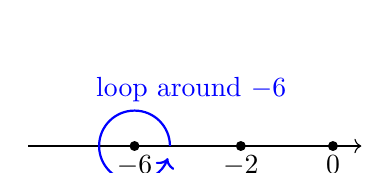
\begin{tikzpicture}[scale=0.9]
	
	\draw[->] (-3.5,0) -- (1.2,0);
	
	\fill (-2,0) circle (2pt);
	\node[below] at (-2,0) {$-6$};
	
	\fill (-0.5,0) circle (2pt);
	\node[below] at (-0.5,0) {$-2$};
	
	\fill (0.8,0) circle (2pt);
	\node[below] at (0.8,0) {$0$};
	
	\draw[thick,blue,->]
	(-1.5,0)
	arc (0:340:0.5);
	
	\node[blue] at (-1.2,0.8)
	{loop around $-6$};
	
\end{tikzpicture}
\]

The loop surrounds the branch value but never passes through it.

This is important because branch values have been removed from the base
space.

\subsection{Clockwise and Counterclockwise Loops}

There are two possible directions:

\begin{itemize}
	\item Counterclockwise,
	\item Clockwise.
\end{itemize}

If \(\gamma\) denotes a loop, then reversing its direction gives

\[
\gamma^{-1}.
\]

The corresponding monodromy permutations are inverses of each other.

For a simple branch point, the monodromy is a transposition

\[
(12).
\]

Since

\[
(12)^{-1}
=
(12),
\]

clockwise and counterclockwise loops produce the same transposition.

For more complicated branch points, the two directions generally yield
different permutations.

\subsection{Why Does a Loop Produce a Permutation?}

Near the critical point \(x=1\),

\[
f(x)
=
-6
+
3(x-1)^2
+
(x-1)^3.
\]

Ignoring higher-order terms gives

\[
y+6
\approx
3(x-1)^2.
\]

Hence

\[
x-1
\approx
\sqrt{\frac{y+6}{3}}.
\]

Write

\[
y+6
=
re^{i\theta}.
\]

Then

\[
x-1
=
\sqrt r\, e^{i\theta/2}.
\]

Suppose \(y\) travels once around the branch value \(-6\).

Then

\[
\theta
:
0
\longrightarrow
2\pi.
\]

Consequently,

\[
x-1
=
\sqrt r\,e^{i\theta/2}
\]

changes into

\[
\sqrt r\,e^{i\pi}
=
-(x-1).
\]

Thus the square root changes sign.

The two roots involved are exchanged:

\[
x_1
\longleftrightarrow
x_2.
\]

This is the transposition

\[
(12).
\]

\subsection{The Physical Picture}

Imagine the three roots moving continuously as \(y\) moves.

Initially,

\[
f^{-1}(0)
=
\{x_1,x_2,x_3\}.
\]

After moving \(y\) once around \(-6\), the roots return to the same set,
but two of them have exchanged positions:

\[
x_1
\leftrightarrow
x_2.
\]

Hence

\[
(x_1,x_2,x_3)
\longmapsto
(x_2,x_1,x_3).
\]

The resulting permutation is

\[
(12).
\]

Similarly, a loop around \(-2\) produces another transposition

\[
(23).
\]

Together these generate

\[
S_3.
\]

\subsection{The Covering-Space Interpretation}

The most important picture is not the graph of

\[
y=x^3-3x-4,
\]

but the three-sheeted covering surface.

Schematically:

\[
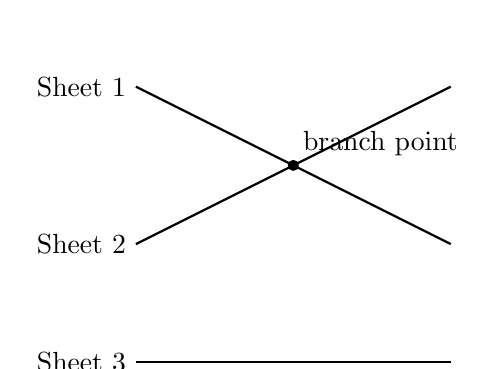
\begin{tikzpicture}[scale=1]
	
	\draw[thick] (-2,1) -- (0,0);
	\draw[thick] (-2,-1) -- (0,0);
	
	\draw[thick] (0,0) -- (2,1);
	\draw[thick] (0,0) -- (2,-1);
	
	\draw[thick] (-2,-2.5) -- (2,-2.5);
	
	\fill (0,0) circle (2pt);
	
	\node[left] at (-2,1) {Sheet 1};
	\node[left] at (-2,-1) {Sheet 2};
	\node[left] at (-2,-2.5) {Sheet 3};
	
	\node[above right] at (0,0) {branch point};
	
\end{tikzpicture}
\]

A loop around a branch value moves us from one sheet to another.

Therefore monodromy measures how the sheets of a covering are globally
glued together.

\[
\boxed{
	\text{Monodromy records how loops permute the sheets of a covering.}
}
\]

For the polynomial

\[
f(x)=x^3-3x-4,
\]

the loops around the branch values produce

\[
(12)
\qquad\text{and}\qquad
(23),
\]

and hence

\[
\boxed{
	\operatorname{Mon}(f)
	=
	S_3.
}
\]

\section{Worked Examples for Problems 8--10}

The purpose of this section is to illustrate the concepts of monodromy,
complex tori, lattice equivalence, and modular transformations through
concrete examples.

\subsection{Example 1: Monodromy of the Square Root Map}

Consider

\[
f(z)=z^2.
\]

Then

\[
w=f(z)=z^2.
\]

The critical point is

\[
z=0,
\]

and the branch value is

\[
w=0.
\]

Choose the base point

\[
w_0=1.
\]

The fibre is

\[
f^{-1}(1)=\{1,-1\}.
\]

Let

\[
\gamma(t)=e^{2\pi it},
\qquad
0\le t\le1.
\]

This loop goes once around the branch value \(0\).

The lifted roots are

\[
z_1(t)=e^{\pi it},
\]

and

\[
z_2(t)=-e^{\pi it}.
\]

At \(t=1\),

\[
z_1(1)=-1,
\]

\[
z_2(1)=1.
\]

Thus the roots exchange positions:

\[
1
\leftrightarrow
-1.
\]

The monodromy permutation is

\[
(12).
\]

Hence

\[
\boxed{
	\operatorname{Mon}(z^2)=S_2.
}
\]

\subsection{Example 2: Monodromy of the Cubic Polynomial}

Consider

\[
f(x)=x^3-3x-4.
\]

Compute

\[
f'(x)=3x^2-3.
\]

Hence

\[
x=\pm1.
\]

The branch values are

\[
f(1)=-6,
\]

and

\[
f(-1)=-2.
\]

Therefore

\[
B=\{-6,-2,\infty\}.
\]

Choose

\[
y_0=0.
\]

The equation

\[
x^3-3x-4=0
\]

has three roots:

\[
x_1\approx2.196,
\]

\[
x_2\approx-1.098+0.786i,
\]

\[
x_3\approx-1.098-0.786i.
\]

A loop around \(-6\) exchanges

\[
x_1
\leftrightarrow
x_2,
\]

giving

\[
(12).
\]

A loop around \(-2\) exchanges

\[
x_2
\leftrightarrow
x_3,
\]

giving

\[
(23).
\]

Therefore

\[
\operatorname{Mon}(f)
=
\langle(12),(23)\rangle.
\]

Since

\[
(12)(23)=(123),
\]

we obtain

\[
\boxed{
	\operatorname{Mon}(f)=S_3.
}
\]

\subsection{Example 3: Constructing a Complex Torus}

Take the lattice

\[
\Lambda
=
\mathbb Z+i\mathbb Z.
\]

Thus

\[
\Lambda
=
\{
m+ni
:
m,n\in\mathbb Z
\}.
\]

The fundamental parallelogram is generated by

\[
1
\qquad\text{and}\qquad
i.
\]

Opposite sides are identified:

\[
z
\sim
z+1,
\]

\[
z
\sim
z+i.
\]

The quotient

\[
\mathbb C/\Lambda
\]

is a torus.

Since the lattice is square, this is called the
\emph{square torus}.

\[
\boxed{
	\mathbb C/(\mathbb Z+i\mathbb Z)
}
\]

is the standard example of a complex torus.

\subsection{Example 4: Equivalent Tori}

Consider

\[
\Lambda_1
=
\mathbb Z+i\mathbb Z.
\]

Let

\[
\Lambda_2
=
2\mathbb Z+2i\mathbb Z.
\]

Then

\[
\Lambda_2
=
2\Lambda_1.
\]

By Problem 9,

\[
\mathbb C/\Lambda_1
\cong
\mathbb C/\Lambda_2.
\]

The conformal equivalence is induced by

\[
F(z)=2z.
\]

Therefore

\[
\boxed{
	\mathbb C/\Lambda_1
	\cong
	\mathbb C/\Lambda_2.
}
\]

\subsection{Example 5: Non-Equivalent Tori}

Consider

\[
\Lambda_1
=
\mathbb Z+i\mathbb Z
\]

and

\[
\Lambda_2
=
\mathbb Z+2i\mathbb Z.
\]

The second lattice is not a complex scalar multiple of the first.

There exists no

\[
c\in\mathbb C^*
\]

such that

\[
\Lambda_2=c\Lambda_1.
\]

Hence

\[
\boxed{
	\mathbb C/\Lambda_1
	\not\cong
	\mathbb C/\Lambda_2.
}
\]

Although both spaces are topological tori, they possess different
complex structures.

\subsection{Example 6: Translation by the Modular Generator \(T\)}

Let

\[
\tau=i.
\]

Apply

\[
T(\tau)=\tau+1.
\]

Then

\[
T(i)=1+i.
\]

The corresponding matrix is

\[
\begin{pmatrix}
	1&1\\
	0&1
\end{pmatrix}.
\]

Since

\[
1+i
=
\frac{1\cdot i+1}{0\cdot i+1},
\]

the lattices

\[
\mathbb Z+i\mathbb Z
\]

and

\[
\mathbb Z+(1+i)\mathbb Z
\]

represent the same complex torus.

Therefore

\[
\boxed{
	i
	\sim
	i+1.
}
\]

\subsection{Example 7: Inversion by the Modular Generator \(S\)}

Let

\[
\tau=i.
\]

Apply

\[
S(\tau)
=
-\frac1\tau.
\]

Then

\[
S(i)
=
-\frac1i
=
i.
\]

Thus \(i\) is fixed by the modular transformation \(S\).

The corresponding matrix is

\[
\begin{pmatrix}
	0&-1\\
	1&0
\end{pmatrix}.
\]

Hence

\[
\boxed{
	i
	=
	-\frac1i.
}
\]

This symmetry explains why the square torus possesses additional
automorphisms.

\subsection{Example 8: The Hexagonal Torus}

Let

\[
\tau
=
e^{2\pi i/3}
=
-\frac12+\frac{\sqrt3}{2}i.
\]

Then

\[
\Lambda
=
\mathbb Z+\mathbb Z\tau.
\]

The lattice forms a triangular grid in the complex plane.

The resulting torus is called the

\begin{itemize}
	\item equianharmonic torus,
	\item hexagonal torus,
	\item triangular torus.
\end{itemize}

It possesses the largest symmetry group among all complex tori.

The corresponding elliptic curve has

\[
j=0.
\]

Therefore

\[
\boxed{
	\tau=e^{2\pi i/3}
}
\]

is one of the most important points in the theory of elliptic curves and
modular forms.

\subsection{Summary Table}

\begin{center}
	\begin{tabular}{|c|c|c|c|}
		\hline
		Example &
		Object &
		Key Result &
		Theory
		\\
		\hline
		1 &
		\(z^2\) &
		\(S_2\) &
		Monodromy
		\\
		\hline
		2 &
		\(x^3-3x-4\) &
		\(S_3\) &
		Monodromy
		\\
		\hline
		3 &
		\(\mathbb C/(\mathbb Z+i\mathbb Z)\) &
		Square Torus &
		Complex Torus
		\\
		\hline
		4 &
		\(2\Lambda\) &
		Equivalent Tori &
		Problem 9
		\\
		\hline
		5 &
		\(\mathbb Z+i\mathbb Z\) vs
		\(\mathbb Z+2i\mathbb Z\) &
		Not Equivalent &
		Problem 9
		\\
		\hline
		6 &
		\(T(\tau)=\tau+1\) &
		Same Torus &
		Modular Group
		\\
		\hline
		7 &
		\(S(\tau)=-1/\tau\) &
		\(i\) Fixed &
		Modular Group
		\\
		\hline
		8 &
		\(e^{2\pi i/3}\) &
		Hexagonal Torus &
		Elliptic Curves
		\\
		\hline
	\end{tabular}
\end{center}

These examples demonstrate the progression

\[
\boxed{
	\text{Monodromy}
}
\Longrightarrow
\boxed{
	\text{Complex Tori}
}
\Longrightarrow
\boxed{
	\text{Modular Transformations}
}
\Longrightarrow
\boxed{
	\text{Elliptic Curves}
}
\]

which is one of the central pathways in modern algebraic geometry,
complex analysis, and number theory.

\section{Problem 11: The Dilogarithm and its Riemann Surface}

\subsection*{Problem statement}

Let
\[
\operatorname{li}_2:D(0,1)\to \mathbb C
\]
be the analytic function given by the series
\[
\operatorname{li}_2(z)=\sum_{n\geq 1}\frac{z^n}{n^2},
\]
so that
\[
z\operatorname{li}_2'(z)=-\log(1-z).
\]
We call \(\operatorname{li}_2\) the dilogarithm function. Let \(\mathcal F\) be the complete analytic function determined by \(\operatorname{li}_2\), and
\[
\pi:R=R_{\mathcal F}\to \mathbb C
\]
its Riemann surface as a covering space of \(\mathbb C\).

\begin{enumerate}
	\item[(i)] Show that for any function element \((f,D)\in \mathcal F\),
	\[
	(zf')'=\frac{1}{1-z}.
	\]
	Deduce that
	\[
	\pi(R)\subset \mathbb C\setminus\{1\}.
	\]
	
	\item[(ii)] Show that
	\[
	\pi(R)=\mathbb C\setminus\{1\},
	\]
	but that \(\pi\) is not a regular covering.
\end{enumerate}

\subsection*{Solution}

For \(|z|<1\),
\[
\operatorname{li}_2(z)=\sum_{n\geq 1}\frac{z^n}{n^2}.
\]
Differentiating term by term gives
\[
\operatorname{li}_2'(z)=\sum_{n\geq 1}\frac{z^{n-1}}{n}.
\]
Hence
\[
z\operatorname{li}_2'(z)
=
\sum_{n\geq 1}\frac{z^n}{n}
=
-\log(1-z).
\]
Differentiating once more,
\[
(z\operatorname{li}_2'(z))'
=
(-\log(1-z))'
=
\frac{1}{1-z}.
\]

Now let \((f,D)\in \mathcal F\) be any analytic continuation of \(\operatorname{li}_2\). Since analytic continuation preserves identities between analytic functions, the same identity holds on \(D\):
\[
(zf')'=\frac{1}{1-z}.
\]

The right-hand side has a pole at \(z=1\). Therefore no analytic branch \(f\) can exist on a neighbourhood of \(1\). Hence
\[
\pi(R)\subset \mathbb C\setminus\{1\}.
\]

We now show the reverse inclusion. The function
\[
\frac{1}{1-z}
\]
is holomorphic on \(\mathbb C\setminus\{1\}\). Therefore
\[
(zf')'
=
\frac{1}{1-z}
\]
can be analytically continued along every path in \(\mathbb C\setminus\{1\}\). Thus the dilogarithm has analytic continuation along every path avoiding \(1\). Hence
\[
\pi(R)=\mathbb C\setminus\{1\}.
\]

It remains to show that the covering is not regular.

The obstruction comes from monodromy. Around \(z=1\),
\[
\log(1-z)
\]
changes by \(2\pi i\). Since
\[
zf'(z)=-\log(1-z),
\]
after one loop around \(1\), the derivative changes by
\[
zf'(z)\mapsto zf'(z)-2\pi i.
\]
Therefore
\[
f'(z)\mapsto f'(z)-\frac{2\pi i}{z}.
\]
Integrating gives
\[
f(z)\mapsto f(z)-2\pi i\log z+\text{constant}.
\]

Thus monodromy around \(1\) introduces a logarithmic term involving \(\log z\). If we then loop around \(0\), this logarithm changes again by \(2\pi i\). Hence the effect of looping around \(1\) and then around \(0\) differs from looping around \(0\) and then around \(1\).

So the monodromy group is non-abelian. In particular, the subgroup corresponding to the covering is not normal in the fundamental group of
\[
\mathbb C\setminus\{0,1\}.
\]
Therefore the covering is not regular.

Hence
\[
\pi:R\to \mathbb C\setminus\{1\}
\]
is a covering, but not a regular covering.

\section{Problem 12: Hyperbolicity of the Twice-Punctured Plane}

\subsection*{Problem statement}

Show that
\[
\mathbb C\setminus\{P,Q\},
\qquad P\neq Q,
\]
is not conformally equivalent to \(\mathbb C\) or \(\mathbb C^*\), and deduce from the uniformization theorem that it is uniformized by the open unit disc \(D\). Show that the same is true for any domain in \(\mathbb C\) whose complement has more than one point.

\subsection*{Solution}

By an affine change of coordinate, we may assume
\[
P=0,\qquad Q=1.
\]
Thus we study
\[
\mathbb C\setminus\{0,1\}.
\]

First, it is not conformally equivalent to \(\mathbb C\). Indeed, \(\mathbb C\) is simply connected, while
\[
\mathbb C\setminus\{0,1\}
\]
is not simply connected. There are nontrivial loops winding around \(0\) and around \(1\).

Second, it is not conformally equivalent to \(\mathbb C^*\). The punctured plane
\[
\mathbb C^*=\mathbb C\setminus\{0\}
\]
has fundamental group
\[
\pi_1(\mathbb C^*)\cong \mathbb Z.
\]
But
\[
\mathbb C\setminus\{0,1\}
\]
has fundamental group the free group on two generators:
\[
\pi_1(\mathbb C\setminus\{0,1\})\cong F_2.
\]
Therefore the two domains cannot be conformally equivalent.

By the uniformization theorem, every simply connected Riemann surface is conformally equivalent to exactly one of
\[
\mathbb P^1,\qquad \mathbb C,\qquad D.
\]
The universal cover of \(\mathbb C\setminus\{0,1\}\) cannot be \(\mathbb P^1\), because \(\mathbb P^1\) is compact and cannot cover a noncompact hyperbolic-type domain. It cannot be \(\mathbb C\), because otherwise the quotient would be conformally equivalent to either \(\mathbb C\) or \(\mathbb C^*\). But we have shown that this is impossible.

Therefore the universal cover must be
\[
D.
\]

Now let \(\Omega\subset \mathbb C\) be any domain whose complement has more than one point. Choose two distinct points
\[
P,Q\in \mathbb C\setminus \Omega.
\]
Then
\[
\Omega\subset \mathbb C\setminus\{P,Q\}.
\]
Since \(\mathbb C\setminus\{P,Q\}\) is hyperbolic, any subdomain of it is also hyperbolic. Hence \(\Omega\) cannot be uniformized by \(\mathbb P^1\) or by \(\mathbb C\).

Therefore \(\Omega\) is also uniformized by the unit disc:
\[
\widetilde{\Omega}\cong D.
\]

\section{Problem 13: Uniformization of Open Riemann Surfaces}

\subsection*{Problem statement}

Let \(R\) be a compact Riemann surface of genus \(g\), and let
\[
p_1,\dots,p_n
\]
be distinct points of \(R\), with \(n\geq 1\). Show that
\[
R\setminus\{p_1,\dots,p_n\}
\]
is uniformized by the open unit disc \(D\) if and only if
\[
2g-2+n>0,
\]
and by \(\mathbb C\) if and only if
\[
2g-2+n=0
\]
or
\[
2g-2+n=-1.
\]

\subsection*{Solution}

Let
\[
X=R\setminus\{p_1,\dots,p_n\}.
\]
The number
\[
2g-2+n
\]
is the negative of the Euler characteristic of \(X\):
\[
\chi(X)=2-2g-n.
\]
Thus
\[
2g-2+n=-\chi(X).
\]

There are three possible simply connected universal covering surfaces:
\[
\mathbb P^1,\qquad \mathbb C,\qquad D.
\]

Since \(X\) is noncompact because \(n\geq 1\), its universal cover cannot be \(\mathbb P^1\). Therefore the universal cover is either
\[
\mathbb C
\]
or
\[
D.
\]

We examine the possible values of \(2g-2+n\).

\subsection*{Case 1: \(2g-2+n=-1\)}

Then
\[
2g-2+n=-1.
\]
Since \(g\geq 0\) and \(n\geq 1\), the only possibility is
\[
g=0,\qquad n=1.
\]
Thus
\[
X=\mathbb P^1\setminus\{\infty\}\cong \mathbb C.
\]
So \(X\) is uniformized by
\[
\mathbb C.
\]

\subsection*{Case 2: \(2g-2+n=0\)}

There are two possibilities:

\[
g=0,\quad n=2,
\]
or
\[
g=1,\quad n=0.
\]

But in the problem \(n\geq 1\), so only
\[
g=0,\qquad n=2
\]
occurs. Then
\[
X=\mathbb P^1\setminus\{0,\infty\}\cong \mathbb C^*.
\]
The universal cover of \(\mathbb C^*\) is
\[
\mathbb C
\]
via
\[
z\mapsto e^z.
\]
Hence \(X\) is uniformized by
\[
\mathbb C.
\]

\subsection*{Case 3: \(2g-2+n>0\)}

All remaining punctured compact Riemann surfaces have negative Euler characteristic:
\[
\chi(X)=2-2g-n<0.
\]
They are hyperbolic. By the uniformization theorem, their universal cover is the unit disc:
\[
\widetilde X\cong D.
\]

Thus
\[
R\setminus\{p_1,\dots,p_n\}
\]
is uniformized by \(D\) exactly when
\[
2g-2+n>0,
\]
and by \(\mathbb C\) exactly when
\[
2g-2+n=0
\]
or
\[
2g-2+n=-1.
\]


\subsection{Final Classification Table}

\begin{center}
	\renewcommand{\arraystretch}{1.3}
	\begin{tabular}{|c|c|c|l|c|}
		\hline
		\textbf{Genus \(g\)} &
		\textbf{Punctures \(n\)} &
		\(\mathbf{2g-2+n}\) &
		\textbf{Surface} &
		\textbf{Universal Cover}
		\\
		\hline
		
		\(0\) & \(1\) & \(-1\)
		&
		\(\mathbb P^1\setminus\{\infty\}\cong\mathbb C\)
		&
		\(\mathbb C\)
		\\
		\hline
		
		\(0\) & \(2\) & \(0\)
		&
		\(\mathbb P^1\setminus\{0,\infty\}\cong\mathbb C^*\)
		&
		\(\mathbb C\)
		\\
		\hline
		
		\(0\) & \(n\ge 3\) & \(>0\)
		&
		Sphere minus \(n\) points
		&
		\(D\)
		\\
		\hline
		
		\(1\) & \(1\) & \(1\)
		&
		Torus minus one point
		&
		\(D\)
		\\
		\hline
		
		\(1\) & \(n\ge 2\) & \(>0\)
		&
		Torus minus \(n\) points
		&
		\(D\)
		\\
		\hline
		
		\(g\ge 2\) & \(n\ge 1\) & \(>0\)
		&
		Higher-genus punctured surface
		&
		\(D\)
		\\
		\hline
		
	\end{tabular}
\end{center}

\bigskip

Therefore,

\[
R\setminus\{p_1,\ldots,p_n\}
\text{ is uniformized by } D
\iff
2g-2+n>0.
\]

Equivalently,

\[
\chi\!\left(R\setminus\{p_1,\ldots,p_n\}\right)
=
2-2g-n
<0.
\]

\bigskip

And

\[
R\setminus\{p_1,\ldots,p_n\}
\text{ is uniformized by } \mathbb C
\iff
2g-2+n=0
\text{ or }
-1.
\]

\bigskip

\subsection{Geometric Interpretation}

The quantity

\[
2g-2+n
=
-\chi\!\left(R\setminus\{p_1,\ldots,p_n\}\right)
\]

measures the complexity of the punctured surface.

\begin{center}
	\begin{tabular}{|c|c|c|}
		\hline
		\(2g-2+n\) &
		Geometry &
		Universal Cover
		\\
		\hline
		
		\(-1\) &
		Parabolic (\(\mathbb C\))
		&
		\(\mathbb C\)
		\\
		\hline
		
		\(0\) &
		Parabolic (\(\mathbb C^*\))
		&
		\(\mathbb C\)
		\\
		\hline
		
		\(>0\) &
		Hyperbolic
		&
		\(D\)
		\\
		\hline
		
	\end{tabular}
\end{center}

\bigskip

Thus the sign of \(2g-2+n\) completely determines the uniformization type of a punctured compact Riemann surface.

\[
\boxed{
	\begin{array}{c}
		2g-2+n\le 0
		\Longrightarrow
		\widetilde{R\setminus\{p_i\}}
		\cong \mathbb C,
		\\[6pt]
		2g-2+n>0
		\Longrightarrow
		\widetilde{R\setminus\{p_i\}}
		\cong D.
	\end{array}
}
\]

\bigskip

\subsection{Relationship Between Problems 11--13}

These three problems form a natural progression in the theory of Riemann surfaces:

\begin{enumerate}
	\item \textbf{Problem 11: The Riemann Surface of the Dilogarithm}
	
	Studies analytic continuation, monodromy, and the construction of a nontrivial Riemann surface associated with a multivalued analytic function.
	
	\item \textbf{Problem 12: Uniformization of the Twice-Punctured Plane}
	
	Introduces hyperbolic Riemann surfaces and shows that
	\(\mathbb C\setminus\{0,1\}\)
	is uniformized by the unit disc.
	
	\item \textbf{Problem 13: Uniformization of Punctured Compact Riemann Surfaces}
	
	Provides the general classification of punctured compact Riemann surfaces according to genus and number of punctures.
\end{enumerate}

\[
\boxed{
	\text{Monodromy}
	\;\Longrightarrow\;
	\text{Hyperbolic Domains}
	\;\Longrightarrow\;
	\text{Uniformization Classification}.
}
\]

\section{Theory Behind Problems 11--13:
	Analytic Continuation, Monodromy, and Uniformization}

Problems 11--13 form a coherent development of some of the central ideas of Riemann surface theory. They connect analytic continuation, monodromy, covering spaces, hyperbolic geometry, and the classification of Riemann surfaces.

The progression is

\[
\text{Analytic Continuation}
\;\Longrightarrow\;
\text{Monodromy}
\;\Longrightarrow\;
\text{Covering Spaces}
\;\Longrightarrow\;
\text{Uniformization}
\;\Longrightarrow\;
\text{Classification}.
\]

\subsection{Function Elements and Analytic Continuation}

A \emph{function element} is a pair

\[
(f,U),
\]

where \(U\subset\mathbb C\) is open and \(f\) is holomorphic on \(U\).

For example,

\[
\left(
\sum_{n=1}^{\infty}\frac{z^n}{n^2},
D(0,1)
\right)
\]

is the initial function element defining the dilogarithm.

\medskip

Suppose

\[
(f,U)
\qquad\text{and}\qquad
(g,V)
\]

are function elements satisfying

\[
f=g
\]

on \(U\cap V\).

Then \(g\) is called an \emph{analytic continuation} of \(f\).

Geometrically one may imagine

\[
U \longrightarrow V
\]

with the function being extended from one region to another while remaining unchanged on the overlap.

\subsection{Complete Analytic Functions}

Starting with a single function element, we may continue it analytically along every possible path.

The collection of all resulting branches forms the \emph{complete analytic function}.

For the dilogarithm,

\[
\operatorname{Li}_2(z)
=
\sum_{n=1}^{\infty}\frac{z^n}{n^2},
\]

the complete analytic function consists of all branches obtained by continuing the series around singular points.

\subsection{Riemann Surfaces of Multivalued Functions}

Many analytic functions are naturally multivalued.

Examples include

\[
\sqrt z,
\qquad
\log z,
\qquad
\operatorname{Li}_2(z).
\]

The idea of a Riemann surface is to replace a multivalued function by a single-valued function on a larger space.

\medskip

For example,

\[
\sqrt z
\]

requires two sheets:

\[
\sqrt z
\quad\leftrightarrow\quad
-\sqrt z.
\]

The logarithm requires infinitely many sheets:

\[
\log z,
\quad
\log z+2\pi i,
\quad
\log z+4\pi i,
\ldots
\]

The complete analytic continuation of the dilogarithm similarly produces a Riemann surface

\[
R_{\mathcal F}
\]

on which the dilogarithm becomes single-valued.

\subsection{Monodromy}

Suppose a branch of a function is analytically continued along a closed loop.

After returning to the starting point, two possibilities arise:

\begin{enumerate}
	\item The original branch is recovered.
	\item A different branch is obtained.
\end{enumerate}

The resulting transformation of branches is called \emph{monodromy}.

\medskip

For example, if one travels once around the origin,

\[
\sqrt z
\longmapsto
-\sqrt z.
\]

Thus the monodromy is nontrivial.

\subsection{The Monodromy Group}

Every loop in the base space determines a permutation of branches.

Consequently there is a representation

\[
\pi_1(X)
\longrightarrow
\mathrm{Perm}(\text{branches}),
\]

called the \emph{monodromy representation}.

The image is the \emph{monodromy group}.

For the dilogarithm, monodromy around \(0\) and \(1\) generates a complicated nonabelian group.

This is the reason that the covering in Problem 11 is not regular.

\subsection{Regular Coverings}

A covering

\[
p:\widetilde X\to X
\]

is called \emph{regular} (or \emph{Galois}) if deck transformations act transitively on every fiber.

Equivalently,

\[
p_*\bigl(\pi_1(\widetilde X)\bigr)
\]

must be a normal subgroup of

\[
\pi_1(X).
\]

Problem 11 provides an important example of a covering that is not regular.

\subsection{The Uniformization Theorem}

One of the most important results in complex analysis is the Uniformization Theorem.

It states that every simply connected Riemann surface is conformally equivalent to exactly one of

\[
\mathbb P^1,
\qquad
\mathbb C,
\qquad
D.
\]

These correspond to the three fundamental geometries:

\begin{center}
	\begin{tabular}{|c|c|c|}
		\hline
		Universal Cover & Geometry & Curvature\\
		\hline
		\(\mathbb P^1\) & Spherical & Positive\\
		\hline
		\(\mathbb C\) & Euclidean & Zero\\
		\hline
		\(D\) & Hyperbolic & Negative\\
		\hline
	\end{tabular}
\end{center}

\subsection{Hyperbolic Riemann Surfaces}

A Riemann surface is called \emph{hyperbolic} if its universal cover is the unit disc

\[
D.
\]

Equivalently, it carries the Poincaré metric.

Typical examples include:

\begin{itemize}
	\item the sphere minus three or more points,
	\item punctured tori,
	\item compact surfaces of genus \(g\ge2\),
	\item domains whose complement contains at least two points.
\end{itemize}

Problem 12 shows that

\[
\mathbb C\setminus\{0,1\}
\]

is hyperbolic.

\subsection{Why Two Punctures Are Special}

Removing one point from the plane gives

\[
\mathbb C^*
=
\mathbb C\setminus\{0\}.
\]

Its universal cover is still

\[
\mathbb C.
\]

However removing two points gives

\[
\mathbb C\setminus\{0,1\},
\]

whose universal cover becomes

\[
D.
\]

This marks the transition from Euclidean to hyperbolic geometry.

\subsection{Genus}

The genus of a compact surface counts handles.

\[
g=0
\]

corresponds to the sphere,

\[
g=1
\]

to the torus,

and

\[
g=2,3,\ldots
\]

to higher-genus surfaces.

\bigskip

\begin{center}
	\begin{tabular}{|c|c|}
		\hline
		Genus & Surface\\
		\hline
		\(0\) & Sphere\\
		\hline
		\(1\) & Torus\\
		\hline
		\(2\) & Double torus\\
		\hline
		\(3\) & Triple torus\\
		\hline
	\end{tabular}
\end{center}

\subsection{Euler Characteristic}

For a compact Riemann surface \(R\) of genus \(g\),

\[
\chi(R)
=
2-2g.
\]

Examples:

\[
\chi(S^2)=2,
\]

\[
\chi(T^2)=0,
\]

\[
\chi(g=2)=-2.
\]

\subsection{Punctures and Euler Characteristic}

Removing a point decreases Euler characteristic by one.

Hence

\[
\chi\!\left(
R\setminus\{p_1,\ldots,p_n\}
\right)
=
2-2g-n.
\]

Equivalently,

\[
2g-2+n
=
-\chi.
\]

This quantity completely determines the uniformization type.

\subsection{Classification by the Quantity \(2g-2+n\)}

\begin{center}
	\begin{tabular}{|c|c|c|}
		\hline
		\(2g-2+n\) & Geometry & Universal Cover\\
		\hline
		\(-1\) & Parabolic & \(\mathbb C\)\\
		\hline
		\(0\) & Parabolic & \(\mathbb C\)\\
		\hline
		\(>0\) & Hyperbolic & \(D\)\\
		\hline
	\end{tabular}
\end{center}

Therefore

\[
2g-2+n>0
\]

if and only if

\[
R\setminus\{p_1,\ldots,p_n\}
\]

is uniformized by the unit disc.

\medskip

And

\[
2g-2+n=0
\quad\text{or}\quad
-1
\]

if and only if the universal cover is

\[
\mathbb C.
\]

\subsection{Conceptual Summary}

The three problems form the chain

\[
\boxed{
	\text{Dilogarithm}
	\Longrightarrow
	\text{Analytic Continuation}
	\Longrightarrow
	\text{Monodromy}
	\Longrightarrow
	\text{Covering Spaces}
	\Longrightarrow
	\text{Uniformization}
	\Longrightarrow
	\text{Hyperbolic Geometry}
	\Longrightarrow
	\text{Classification of Open Riemann Surfaces}.
}
\]

This sequence leads naturally to many advanced topics:

\begin{itemize}
	\item Fuchsian groups,
	\item automorphic functions,
	\item modular curves,
	\item elliptic curves,
	\item Teichmüller theory,
	\item algebraic curves,
	\item moduli spaces of Riemann surfaces.
\end{itemize}
\section{Examples for Problems 11--13}

\subsection{Example 1: Analytic Continuation of the Logarithm}

Before studying the dilogarithm, it is useful to recall the simpler example of the logarithm.

Start with the principal branch

\[
\Log z
\]

defined on

\[
\mathbb C\setminus (-\infty,0].
\]

It satisfies

\[
(\Log z)'=\frac1z.
\]

Now continue \(\Log z\) once around the origin. After one full turn,

\[
z\mapsto e^{2\pi i}z=z,
\]

but the logarithm changes by

\[
\Log z \mapsto \Log z+2\pi i.
\]

Thus logarithm has infinitely many branches:

\[
\Log z+2\pi i k,
\qquad k\in\mathbb Z.
\]

Its Riemann surface is an infinite-sheeted covering of

\[
\mathbb C^*.
\]

The universal covering map is

\[
\exp:\mathbb C\to\mathbb C^*.
\]

\[
w\mapsto e^w.
\]

Therefore

\[
\mathbb C
\]

is the Riemann surface on which \(\log z\) becomes single-valued.

\subsection{Example 2: Monodromy of the Square Root}

Consider

\[
f(z)=\sqrt z.
\]

Start at a point \(z_0\neq 0\). Choose one value of the square root.

Now travel once around \(0\). Write

\[
z=re^{i\theta}.
\]

Then

\[
\sqrt z=\sqrt r e^{i\theta/2}.
\]

After one loop,

\[
\theta\mapsto \theta+2\pi.
\]

Hence

\[
\sqrt r e^{i\theta/2}
\mapsto
\sqrt r e^{i(\theta+2\pi)/2}
=
-\sqrt r e^{i\theta/2}.
\]

So

\[
\sqrt z\mapsto -\sqrt z.
\]

After two loops,

\[
-\sqrt z\mapsto \sqrt z.
\]

Thus the monodromy group has two elements:

\[
\mathbb Z/2\mathbb Z.
\]

This is a regular two-sheeted covering of

\[
\mathbb C^*.
\]

\subsection{Example 3: First Monodromy of the Dilogarithm}

The dilogarithm satisfies

\[
z\operatorname{Li}_2'(z)
=
-\log(1-z).
\]

Therefore

\[
\operatorname{Li}_2'(z)
=
-\frac{\log(1-z)}{z}.
\]

Now continue around \(z=1\).

The logarithm changes by

\[
\log(1-z)
\mapsto
\log(1-z)+2\pi i.
\]

Therefore

\[
\operatorname{Li}_2'(z)
\mapsto
\operatorname{Li}_2'(z)
-
\frac{2\pi i}{z}.
\]

Integrating gives

\[
\operatorname{Li}_2(z)
\mapsto
\operatorname{Li}_2(z)
-
2\pi i \log z
+
C.
\]

Thus going around \(1\) does not merely add a constant. It introduces the logarithm \(\log z\).

This is why the monodromy of the dilogarithm is more complicated than the monodromy of \(\log z\).

\subsection{Example 4: Noncommuting Loops for the Dilogarithm}

Let

\[
A
\]

be a loop around \(0\), and let

\[
B
\]

be a loop around \(1\).

For the logarithm,

\[
\log z
\mapsto
\log z+2\pi i
\]

under the loop \(A\).

But after applying \(B\), the dilogarithm branch contains a term

\[
-2\pi i\log z.
\]

Now applying \(A\) changes this term:

\[
-2\pi i\log z
\mapsto
-2\pi i(\log z+2\pi i).
\]

Hence an additional constant appears:

\[
-2\pi i\cdot 2\pi i
=
4\pi^2.
\]

Therefore

\[
AB\neq BA
\]

as transformations of branches.

This shows that the monodromy group is nonabelian.

Consequently the Riemann surface of the dilogarithm is not a regular covering.

\subsection{Example 5: The Plane \(\mathbb C\)}

The complex plane

\[
\mathbb C
\]

is simply connected.

Therefore its universal cover is itself:

\[
\widetilde{\mathbb C}
\cong
\mathbb C.
\]

It has Euclidean geometry.

In the notation of Problem 13, this is

\[
\mathbb P^1\setminus\{\infty\}.
\]

Here

\[
g=0,
\qquad
n=1.
\]

Thus

\[
2g-2+n
=
0-2+1
=
-1.
\]

So this is one of the parabolic cases.

\subsection{Example 6: The Punctured Plane \(\mathbb C^*\)}

Consider

\[
\mathbb C^*
=
\mathbb C\setminus\{0\}.
\]

It is not simply connected, since loops can wind around \(0\).

Its fundamental group is

\[
\pi_1(\mathbb C^*)
\cong
\mathbb Z.
\]

The universal covering map is

\[
\exp:\mathbb C\to\mathbb C^*.
\]

Indeed,

\[
e^{w+2\pi i}=e^w.
\]

Therefore the deck transformation group is

\[
w\mapsto w+2\pi i k,
\qquad k\in\mathbb Z.
\]

In Problem 13 this corresponds to

\[
\mathbb P^1\setminus\{0,\infty\}.
\]

Here

\[
g=0,
\qquad
n=2.
\]

Thus

\[
2g-2+n
=
0-2+2
=
0.
\]

Therefore

\[
\widetilde{\mathbb C^*}
\cong
\mathbb C.
\]

\subsection{Example 7: The Twice-Punctured Plane}

Consider

\[
\mathbb C\setminus\{0,1\}.
\]

This surface has two independent loops:

\[
\gamma_0
\]

around \(0\), and

\[
\gamma_1
\]

around \(1\).

Therefore

\[
\pi_1(\mathbb C\setminus\{0,1\})
\cong
F_2,
\]

the free group on two generators.

This is already much more complicated than

\[
\pi_1(\mathbb C^*)\cong \mathbb Z.
\]

The universal cover is not \(\mathbb C\), but the unit disc:

\[
\widetilde{\mathbb C\setminus\{0,1\}}
\cong
D.
\]

This is the first basic example of a hyperbolic plane domain.

\subsection{Example 8: Sphere Minus Three Points}

Consider

\[
X
=
\mathbb P^1\setminus\{0,1,\infty\}.
\]

This is conformally equivalent to

\[
\mathbb C\setminus\{0,1\}.
\]

Here

\[
g=0,
\qquad
n=3.
\]

Then

\[
2g-2+n
=
0-2+3
=
1>0.
\]

Hence

\[
\widetilde X
\cong
D.
\]

This is one of the most important hyperbolic Riemann surfaces.

It appears in:

\begin{itemize}
	\item modular forms,
	\item hypergeometric functions,
	\item monodromy theory,
	\item algebraic curves,
	\item dessins d'enfants.
\end{itemize}

\subsection{Example 9: Torus Minus One Point}

Let \(R\) be a compact torus:

\[
R=\mathbb C/\Lambda.
\]

Remove one point:

\[
X=R\setminus\{p\}.
\]

Here

\[
g=1,
\qquad
n=1.
\]

Therefore

\[
2g-2+n
=
2-2+1
=
1>0.
\]

Hence

\[
\widetilde X
\cong
D.
\]

This is important: the compact torus itself has universal cover

\[
\mathbb C,
\]

but after removing one point, the surface becomes hyperbolic and has universal cover

\[
D.
\]

So one puncture changes the geometry from Euclidean to hyperbolic.

\subsection{Example 10: Compact Torus Without Punctures}

Let

\[
R=\mathbb C/\Lambda
\]

be a compact torus.

Then

\[
g=1,
\qquad
n=0.
\]

Although Problem 13 assumes \(n\ge1\), this case is useful for comparison.

We have

\[
2g-2+n
=
2-2+0
=
0.
\]

The universal cover is

\[
\mathbb C.
\]

Thus compact tori are Euclidean Riemann surfaces.

\subsection{Example 11: Genus Two Surface}

Let \(R\) be a compact Riemann surface of genus

\[
g=2.
\]

With no punctures,

\[
2g-2
=
4-2
=
2>0.
\]

Thus the compact genus two surface is already hyperbolic:

\[
\widetilde R
\cong
D.
\]

If we remove \(n\ge1\) points, then

\[
2g-2+n
=
2+n>0.
\]

So the punctured surface is also hyperbolic.

\subsection{Example 12: General Sphere Minus \(n\) Points}

Let

\[
X=\mathbb P^1\setminus\{p_1,\dots,p_n\}.
\]

Then

\[
g=0.
\]

Therefore

\[
2g-2+n
=
n-2.
\]

So:

\[
n=1
\quad\Rightarrow\quad
n-2=-1,
\]

and

\[
X\cong\mathbb C.
\]

\[
n=2
\quad\Rightarrow\quad
n-2=0,
\]

and

\[
X\cong\mathbb C^*.
\]

\[
n\ge3
\quad\Rightarrow\quad
n-2>0,
\]

and

\[
\widetilde X\cong D.
\]

Thus the sphere becomes hyperbolic exactly after removing at least three points.

\subsection{Example 13: General Genus \(g\) Surface With \(n\) Punctures}

Let

\[
X=R\setminus\{p_1,\dots,p_n\}.
\]

Then

\[
\chi(X)=2-2g-n.
\]

The key number is

\[
-\chi(X)=2g-2+n.
\]

If

\[
2g-2+n>0,
\]

then

\[
X
\]

is hyperbolic and

\[
\widetilde X\cong D.
\]

If

\[
2g-2+n=0
\]

or

\[
2g-2+n=-1,
\]

then

\[
\widetilde X\cong\mathbb C.
\]

\subsection{Deep Example: Why \(\mathbb C\setminus\{0,1\}\) Is Hyperbolic}

The plane minus one point,

\[
\mathbb C^*,
\]

is covered by

\[
\mathbb C
\]

via

\[
z\mapsto e^z.
\]

But the plane minus two points,

\[
\mathbb C\setminus\{0,1\},
\]

cannot be covered by \(\mathbb C\).

If it were covered by \(\mathbb C\), then it would be a quotient

\[
\mathbb C/\Gamma
\]

by a group of affine transformations acting freely and properly discontinuously.

The possible quotients of \(\mathbb C\) are essentially:

\[
\mathbb C,
\qquad
\mathbb C^*,
\qquad
\text{tori}.
\]

But

\[
\mathbb C\setminus\{0,1\}
\]

is none of these.

Therefore its universal cover must be

\[
D.
\]

This shows that adding just one more puncture changes the conformal type completely.

\subsection{Deep Example: Euler Characteristic Controls Geometry}

For

\[
X=R\setminus\{p_1,\dots,p_n\},
\]

we have

\[
\chi(X)=2-2g-n.
\]

There are three geometric possibilities:

\[
\chi(X)>0,
\qquad
\chi(X)=0,
\qquad
\chi(X)<0.
\]

But since \(n\ge1\), the positive case does not occur except before puncturing.

So we get:

\[
\chi(X)=1
\quad\Longleftrightarrow\quad
X\cong \mathbb C,
\]

\[
\chi(X)=0
\quad\Longleftrightarrow\quad
X\cong \mathbb C^*,
\]

\[
\chi(X)<0
\quad\Longleftrightarrow\quad
X \text{ is hyperbolic}.
\]

Equivalently:

\[
2g-2+n<0
\quad\Longleftrightarrow\quad
\mathbb C,
\]

\[
2g-2+n=0
\quad\Longleftrightarrow\quad
\mathbb C^*,
\]

\[
2g-2+n>0
\quad\Longleftrightarrow\quad
D.
\]

\subsection{Summary Table of Examples}

\begin{center}
	\renewcommand{\arraystretch}{1.3}
	\begin{tabular}{|c|c|c|c|c|}
		\hline
		Surface & \(g\) & \(n\) & \(2g-2+n\) & Universal Cover\\
		\hline
		\(\mathbb C\) & \(0\) & \(1\) & \(-1\) & \(\mathbb C\)\\
		\hline
		\(\mathbb C^*\) & \(0\) & \(2\) & \(0\) & \(\mathbb C\)\\
		\hline
		\(\mathbb C\setminus\{0,1\}\) & \(0\) & \(3\) & \(1\) & \(D\)\\
		\hline
		Torus & \(1\) & \(0\) & \(0\) & \(\mathbb C\)\\
		\hline
		Torus minus one point & \(1\) & \(1\) & \(1\) & \(D\)\\
		\hline
		Genus \(2\) compact surface & \(2\) & \(0\) & \(2\) & \(D\)\\
		\hline
		Genus \(2\) minus \(n\) points & \(2\) & \(n\ge1\) & \(2+n\) & \(D\)\\
		\hline
	\end{tabular}
\end{center}

\section{Diagrams and Visualizations for Problems 11--13}

\subsection{Analytic Continuation Around the Origin}

\begin{center}
	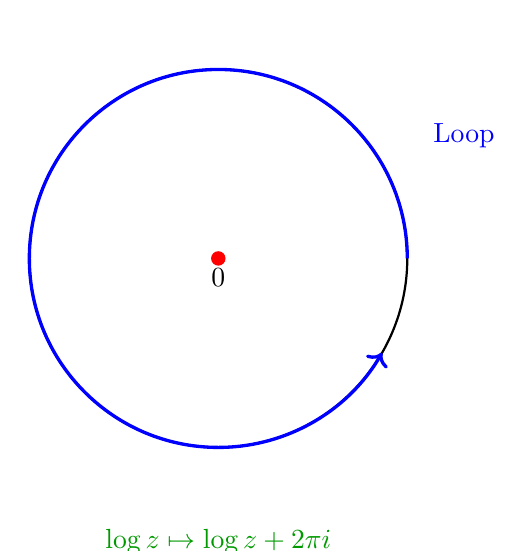
\begin{tikzpicture}[scale=1.2]
		
		\draw[thick] (0,0) circle (2);
		
		\filldraw[red] (0,0) circle (2pt);
		\node[below] at (0,0) {$0$};
		
		\draw[blue,very thick,->]
		(2,0)
		arc(0:330:2);
		
		\node[blue] at (2.6,1.3)
		{Loop};
		
		\node[green!60!black]
		at (0,-3)
		{$\log z \mapsto \log z + 2\pi i$};
		
	\end{tikzpicture}
\end{center}

\subsection{The Two Sheets of the Square Root}

\begin{center}
	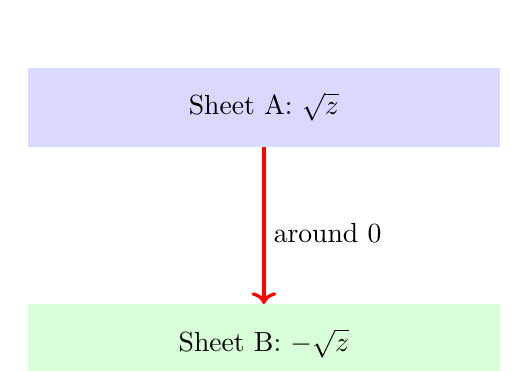
\begin{tikzpicture}
		
		\fill[blue!15]
		(-3,1) rectangle (3,2);
		
		\fill[green!15]
		(-3,-2) rectangle (3,-1);
		
		\node at (0,1.5)
		{Sheet A: $\sqrt z$};
		
		\node at (0,-1.5)
		{Sheet B: $-\sqrt z$};
		
		\draw[red,very thick,->]
		(0,1) -- (0,-1);
		
		\node[right]
		at (0,-0.1)
		{around $0$};
		
	\end{tikzpicture}
\end{center}

\subsection{The Logarithm Riemann Surface}

\begin{center}
	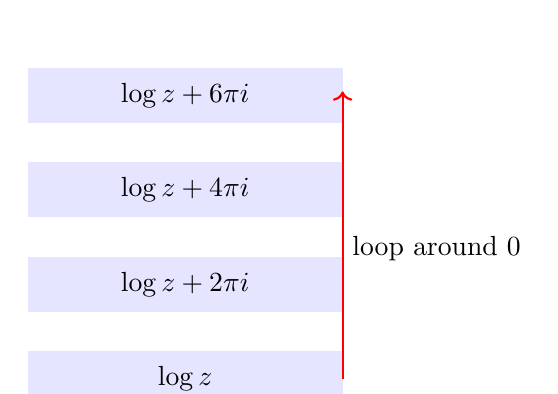
\begin{tikzpicture}
		
		\foreach \y/\txt in
		{
			0/{$\log z$},
			1.2/{$\log z+2\pi i$},
			2.4/{$\log z+4\pi i$},
			3.6/{$\log z+6\pi i$}
		}
		{
			\fill[blue!10]
			(-2,\y) rectangle (2,\y+0.7);
			
			\node at (0,\y+0.35) {\txt};
		}
		
		\draw[red,thick,->]
		(2,0.35)
		--
		(2,4);
		
		\node[right]
		at (2,2)
		{loop around $0$};
		
	\end{tikzpicture}
\end{center}

\subsection{Two Independent Loops}

\begin{center}
	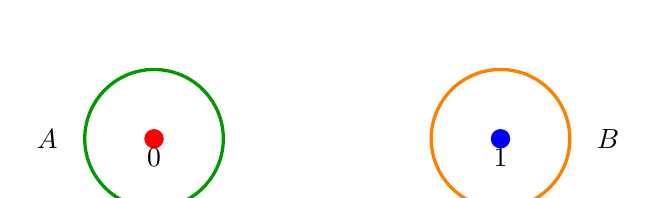
\begin{tikzpicture}[scale=1.1]
		
		\filldraw[red]
		(-2,0) circle (3pt);
		
		\filldraw[blue]
		(2,0) circle (3pt);
		
		\node[below]
		at (-2,0) {$0$};
		
		\node[below]
		at (2,0) {$1$};
		
		\draw[green!60!black,very thick]
		(-2,0)
		circle (0.8);
		
		\draw[orange,very thick]
		(2,0)
		circle (0.8);
		
		\node[left]
		at (-3,0)
		{$A$};
		
		\node[right]
		at (3,0)
		{$B$};
		
	\end{tikzpicture}
\end{center}

\subsection{The Three Simply Connected Surfaces}

\begin{center}
	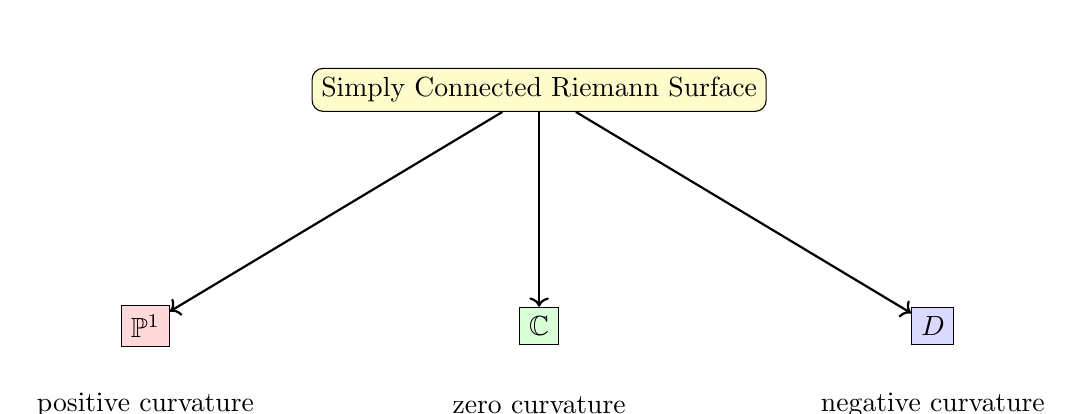
\begin{tikzpicture}[node distance=3cm]
		
		\node[
		draw,
		rounded corners,
		fill=yellow!20
		]
		(U)
		{Simply Connected Riemann Surface};
		
		\node[
		draw,
		fill=red!15
		]
		(S)
		at (-5,-3)
		{$\mathbb P^1$};
		
		\node[
		draw,
		fill=green!15
		]
		(C)
		at (0,-3)
		{$\mathbb C$};
		
		\node[
		draw,
		fill=blue!15
		]
		(D)
		at (5,-3)
		{$D$};
		
		\draw[thick,->] (U)--(S);
		\draw[thick,->] (U)--(C);
		\draw[thick,->] (U)--(D);
		
		\node
		at (-5,-4)
		{positive curvature};
		
		\node
		at (0,-4)
		{zero curvature};
		
		\node
		at (5,-4)
		{negative curvature};
		
	\end{tikzpicture}
\end{center}
\subsection{Classification of Punctured Surfaces}

\begin{center}
	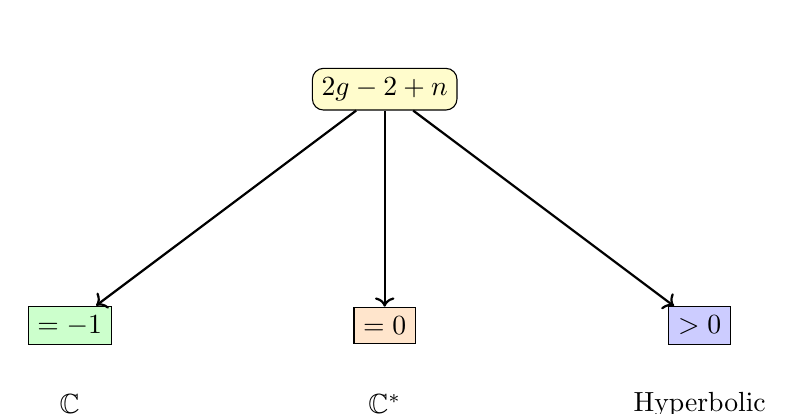
\begin{tikzpicture}[node distance=2.5cm]
		
		\node[
		draw,
		rounded corners,
		fill=yellow!20
		]
		(A)
		{$2g-2+n$};
		
		\node[
		draw,
		fill=green!20
		]
		(B)
		at (-4,-3)
		{$=-1$};
		
		\node[
		draw,
		fill=orange!20
		]
		(C)
		at (0,-3)
		{$=0$};
		
		\node[
		draw,
		fill=blue!20
		]
		(D)
		at (4,-3)
		{$>0$};
		
		\draw[thick,->] (A)--(B);
		\draw[thick,->] (A)--(C);
		\draw[thick,->] (A)--(D);
		
		\node
		at (-4,-4)
		{$\mathbb C$};
		
		\node
		at (0,-4)
		{$\mathbb C^*$};
		
		\node
		at (4,-4)
		{Hyperbolic};
		
	\end{tikzpicture}
\end{center}

\subsection{Genus and Geometry}

\begin{center}
	
	\begin{tabular}{|c|c|c|}
		\hline
		Genus & Picture & Universal Cover\\
		\hline
		0 & Sphere & $\mathbb P^1$\\
		\hline
		1 & Torus & $\mathbb C$\\
		\hline
		2 & Double Torus & $D$\\
		\hline
		3 & Triple Torus & $D$\\
		\hline
	\end{tabular}
	
\end{center}

\subsection{Concept Map}

\begin{center}
	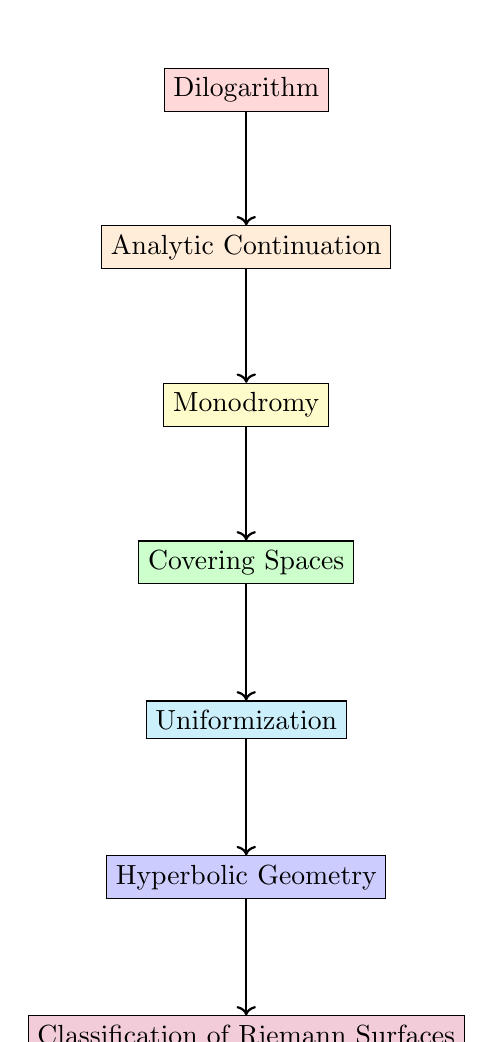
\begin{tikzpicture}[node distance=2cm]
		
		\node[draw,fill=red!15] (A)
		{Dilogarithm};
		
		\node[draw,fill=orange!15] (B)
		[below of=A]
		{Analytic Continuation};
		
		\node[draw,fill=yellow!20] (C)
		[below of=B]
		{Monodromy};
		
		\node[draw,fill=green!20] (D)
		[below of=C]
		{Covering Spaces};
		
		\node[draw,fill=cyan!20] (E)
		[below of=D]
		{Uniformization};
		
		\node[draw,fill=blue!20] (F)
		[below of=E]
		{Hyperbolic Geometry};
		
		\node[draw,fill=purple!20] (G)
		[below of=F]
		{Classification of Riemann Surfaces};
		
		\draw[thick,->] (A)--(B);
		\draw[thick,->] (B)--(C);
		\draw[thick,->] (C)--(D);
		\draw[thick,->] (D)--(E);
		\draw[thick,->] (E)--(F);
		\draw[thick,->] (F)--(G);
		
	\end{tikzpicture}
\end{center}

\section{Connections to Other Areas of Mathematics}

Problems 11--13 lie at the intersection of several major branches of modern mathematics. The ideas of analytic continuation, monodromy, covering spaces, and uniformization reappear throughout complex analysis, topology, algebraic geometry, differential geometry, number theory, and mathematical physics.

\subsection{Connection with Complex Analysis}

The starting point is the theory of holomorphic functions.

Analytic continuation extends locally defined holomorphic functions beyond their original domain of convergence. The dilogarithm in Problem 11 is a classical example: its power series converges only in the unit disc, yet the function itself possesses a much larger analytic continuation.

Many important special functions arise in exactly this way:

\[
\log z,
\qquad
\sqrt z,
\qquad
\arcsin z,
\qquad
\Gamma(z),
\qquad
\operatorname{Li}_s(z).
\]

The study of their singularities naturally leads to monodromy and Riemann surfaces.

\subsection{Connection with Covering Space Theory}

Every Riemann surface can be studied through its universal covering space.

Problem 11 constructs a covering from analytic continuation.

Problem 12 studies the universal covering of

\[
\mathbb C\setminus\{0,1\},
\]

while Problem 13 classifies coverings of punctured compact surfaces.

This connects directly to algebraic topology:

\[
\pi_1(X)
\longleftrightarrow
\text{covering spaces}.
\]

Fundamental groups classify connected coverings.

For example,

\[
\pi_1(\mathbb C^*)
\cong
\mathbb Z,
\]

while

\[
\pi_1(\mathbb C\setminus\{0,1\})
\cong
F_2.
\]

Thus topology controls the analytic behavior of functions.

\subsection{Connection with Fundamental Groups}

Monodromy may be viewed as a representation

\[
\pi_1(X)
\longrightarrow
\operatorname{Aut}(\text{branches}).
\]

Thus every multivalued analytic function produces a representation of the fundamental group.

This idea generalizes to:

\begin{itemize}
	\item differential equations,
	\item local systems,
	\item vector bundles,
	\item flat connections,
	\item algebraic geometry.
\end{itemize}

The modern theory of monodromy representations begins with precisely the examples studied in Problem 11.

\subsection{Connection with Differential Equations}

Many differential equations possess multivalued solutions.

Classical examples include:

\[
z(1-z)y''+[c-(a+b+1)z]y'-aby=0,
\]

the hypergeometric equation.

Its solutions have singularities at

\[
0,\quad 1,\quad \infty,
\]

exactly the same points appearing in Problem 12.

Analytic continuation around these singularities generates a monodromy group.

Thus the theory of differential equations naturally leads to Riemann surfaces and monodromy.

\subsection{Connection with Hypergeometric Functions}

The hypergeometric function

\[
{}_2F_1(a,b;c;z)
\]

is one of the most important special functions in mathematics.

Its analytic continuation is controlled by loops around

\[
0,\quad 1,\quad \infty.
\]

Consequently,

\[
\mathbb P^1\setminus\{0,1,\infty\}
\]

plays a central role.

This is exactly the surface that appears in Problem 12.

Many classical functions are special cases of hypergeometric functions.

\subsection{Connection with Hyperbolic Geometry}

Problem 12 introduces hyperbolic surfaces.

The universal cover

\[
D
\]

carries the Poincaré metric

\[
ds^2=
\frac{4|dz|^2}
{(1-|z|^2)^2}.
\]

This metric has constant negative curvature

\[
K=-1.
\]

Consequently every hyperbolic Riemann surface inherits a hyperbolic geometry.

Problem 13 can therefore be interpreted as a classification of which punctured surfaces admit hyperbolic metrics.

\subsection{Connection with Fuchsian Groups}

Whenever a Riemann surface has universal cover

\[
D,
\]

it can be represented as

\[
D/\Gamma,
\]

where

\[
\Gamma
\]

is a discrete subgroup of Möbius transformations preserving the unit disc.

Such groups are called Fuchsian groups.

Thus every hyperbolic surface may be described by a group action.

This provides a bridge between geometry and group theory.

\subsection{Connection with Algebraic Curves}

Compact Riemann surfaces are equivalent to smooth projective algebraic curves over \(\mathbb C\).

Examples:

\[
y^2=x^3-x
\]

defines an elliptic curve.

\[
y^2=x^5-1
\]

defines a genus-two curve.

Thus Problem 13 is simultaneously a classification statement about algebraic curves.

The quantity

\[
2g-2+n
\]

also appears throughout algebraic geometry.

\subsection{Connection with Elliptic Curves}

Elliptic curves are compact Riemann surfaces of genus

\[
g=1.
\]

Every elliptic curve has the form

\[
\mathbb C/\Lambda,
\]

where

\[
\Lambda
=
\mathbb Z\omega_1+\mathbb Z\omega_2.
\]

Thus its universal cover is

\[
\mathbb C.
\]

This is precisely one of the Euclidean cases appearing in Problem 13.

Removing even a single point changes the geometry:

\[
(\mathbb C/\Lambda)\setminus\{p\}
\]

becomes hyperbolic and is uniformized by

\[
D.
\]

\subsection{Connection with Modular Curves}

One of the most important examples in modern mathematics is

\[
\mathbb H/\operatorname{SL}(2,\mathbb Z),
\]

where \(\mathbb H\) denotes the upper half-plane.

This quotient is closely related to

\[
\mathbb P^1\setminus\{0,1,\infty\}.
\]

Thus the geometry of modular curves originates from exactly the hyperbolic surfaces studied in Problems 12 and 13.

\subsection{Connection with Teichmüller Theory}

Teichmüller theory studies all possible complex structures on a given topological surface.

Every compact surface of genus

\[
g\ge2
\]

admits hyperbolic geometry.

The corresponding moduli space describes all such structures.

Problems 12 and 13 provide the first examples of surfaces lying inside Teichmüller theory.

\subsection{Connection with Algebraic Topology}

The classification

\[
2g-2+n
\]

depends only on topology.

The quantity

\[
\chi
=
2-2g-n
\]

is the Euler characteristic.

Thus topology determines:

\begin{itemize}
	\item the universal cover,
	\item the geometry,
	\item the existence of hyperbolic metrics,
	\item the structure of the fundamental group.
\end{itemize}

This is a remarkable interaction between topology and complex analysis.

\subsection{Connection with Number Theory}

The dilogarithm appearing in Problem 11 occurs throughout modern number theory.

It appears in:

\begin{itemize}
	\item algebraic \(K\)-theory,
	\item regulators,
	\item polylogarithms,
	\item special values of zeta functions,
	\item Bloch groups.
\end{itemize}

The study of its monodromy is an active area of research.

\subsection{Connection with Mathematical Physics}

Polylogarithms, including the dilogarithm, occur in:

\begin{itemize}
	\item quantum field theory,
	\item Feynman integrals,
	\item statistical mechanics,
	\item conformal field theory,
	\item string theory.
\end{itemize}

The monodromy of these functions often encodes physical information about the system.

\subsection{Conceptual Overview}

The ideas of Problems 11--13 connect to a surprisingly large part of mathematics:

\[
\boxed{
	\begin{array}{c}
		\text{Dilogarithm} \\
		\Downarrow \\
		\text{Analytic Continuation} \\
		\Downarrow \\
		\text{Monodromy} \\
		\Downarrow \\
		\text{Covering Spaces} \\
		\Downarrow \\
		\text{Fundamental Groups} \\
		\Downarrow \\
		\text{Uniformization} \\
		\Downarrow \\
		\text{Hyperbolic Geometry} \\
		\Downarrow \\
		\text{Algebraic Curves} \\
		\Downarrow \\
		\text{Modular Curves and Teichmüller Theory}
	\end{array}
}
\]

Thus Problems 11--13 form a gateway from elementary complex analysis to some of the deepest theories in modern mathematics.

\end{document}

